\documentclass[12pt]{article}
\usepackage{amssymb}
\usepackage[UTF8]{ctex}
\usepackage{geometry}
\usepackage{units}
\usepackage{pifont}
\geometry{
	a4paper,
	total={150mm,237mm},
	left=30mm,
	top=27mm,
	}
\usepackage{amsmath}
\usepackage{enumerate}
\usepackage{lipsum}
\usepackage{graphicx}
\usepackage{hyperref}
\usepackage{indentfirst}
\usepackage[graphicx]{realboxes}
\usepackage{booktabs}
\usepackage{cases}
\usepackage{subfig}  
\usepackage{float}
\usepackage{xcolor}
\setlength{\parindent}{2em}
\title{Lab5}
\author{姓名:陈锐林,学号:21307130148}
\date{\today}

\begin{document}
\maketitle
\begin{Large}
	\noindent 一、实验思路\par
\end{Large}
1.这次实验出发点是对xv6的fork进行改进,达到高效、简洁、低耗的目标。\par
2.大体思路如下:(1)当fork时(调用uvmcopy时),让父子结点映射到同一目标;(2)当遇到写操作,usertrap的时候;对这些内容进行拷贝;(3)完善设置:
需要同时对kfree/kalloc/copyout进行修改;更新PTE;并基于当前共享这一物理页的进程数作出判断;为1时要特殊处理。\par
3.由hint/之前的实验可以得到的借助: (1)判断是否存在这一现象可以设置RISC-V的RSW位;(2)mappages函数作映射;(3)walk/walkaddr函数作地址转换;(4)r\_scause函数返回错误码;(5)可以利用spinlock完成计数值的更改;(6)PGROUNDDOWN等函数获取页表信息。\\


\begin{Large}
	\noindent 二、具体实现\par
\end{Large}
1.在riscv.h中先设置PTE位,其中取1<<8为PTE\_COW,表示进行了COW操作。\par
2.修改uvmcopy,主要修改是删除了原先用于分配的char *mem;并利用mappages将父子结点映射。其中根据计数的规则,fork后要及时修改计数,add\_ref放在后面实现。
\begin{figure}[H]
    \centering
    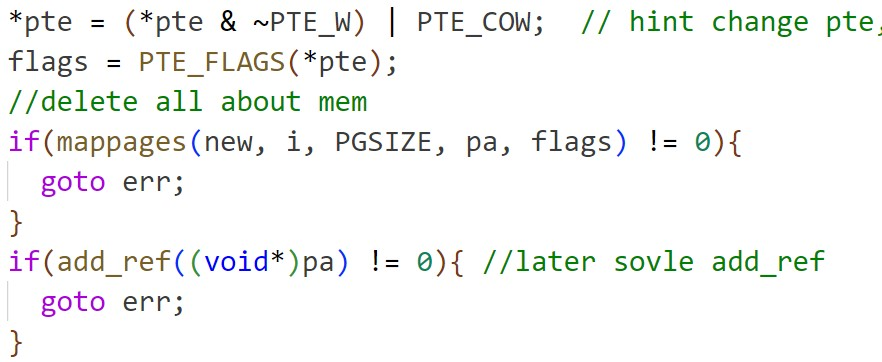
\includegraphics[height=4.5cm,width=8cm]{lab5-1.jpg}
\end{figure}\par
3.在kalloc.c中完成定义,具体来说是以下几步:
\newpage
\noindent(1)仿照kmem结构体,完成对计数结构体ref的定义;其中计数为1数组,大小应是(地址空间大小/页大小)最大页数。并在kinit里初始化锁;
\begin{figure*}[!h]
    \centering
    \subfloat[struct ref]{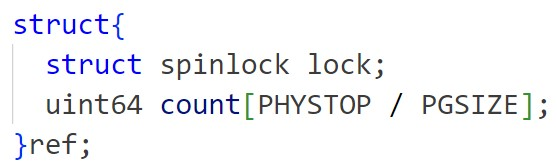
\includegraphics[width=5cm,height=3cm]{lab5-3.jpg} \label{X}}
    \hfill
    \subfloat[kinit]{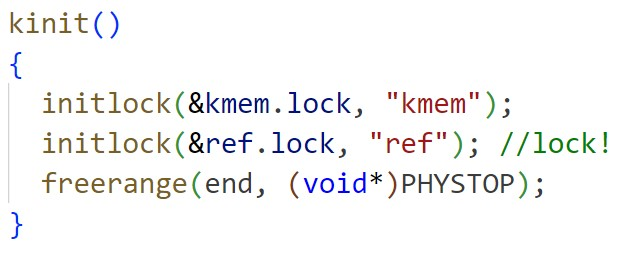
\includegraphics[width=5cm,height=3.7cm]{lab5-2.jpg} \label{Y}}
\end{figure*}\\
\noindent(2)在kalloc里初始化count数组为全1。
\begin{figure}[H]
    \centering
    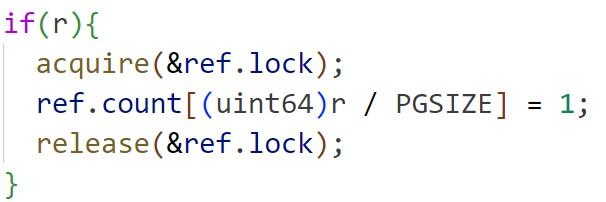
\includegraphics[height=3.5cm,width=6cm]{lab5-6.jpg}
\end{figure}
\noindent(3)在kfree里完成对当前页面ref--,以及在ref为0时,真正free。
\begin{figure}[H]
    \centering
    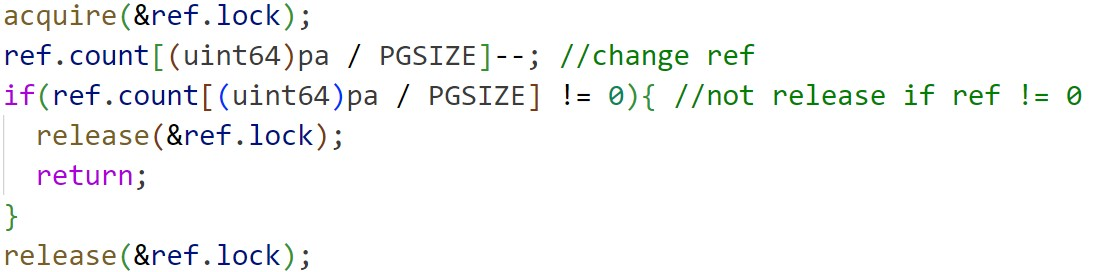
\includegraphics[height=4cm,width=9cm]{lab5-5.jpg}
\end{figure}
\noindent(4)还需要注意freearange函数,对于从pa\_start到pa\_end的页面,需要都初始化计数器为1,避免0-1=大正数。\\
\begin{figure}[H]
    \centering
    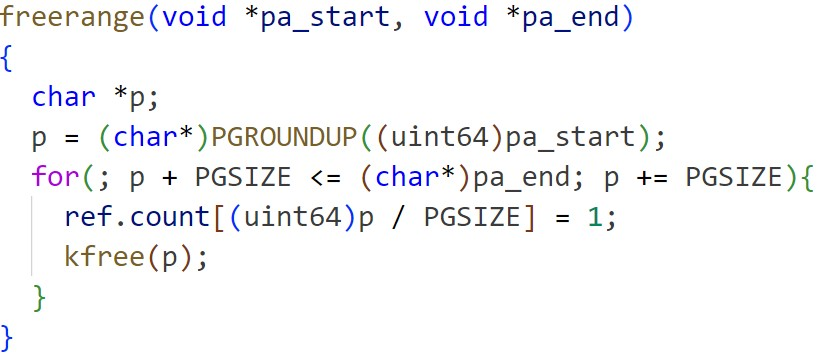
\includegraphics[height=4cm,width=7cm]{lab5-4.jpg}
\end{figure}
\newpage
\noindent(5)完成add\_ref函数的定义,其实逻辑很简单,就是count[pa/pgsize]++;但是需要补一下判断,此时的pa是不是还在地址空间内,并且这个pa应该是整除PGSIZE的。
还有get\_ref,简单的接口函数。
\begin{figure}[H]
    \centering
    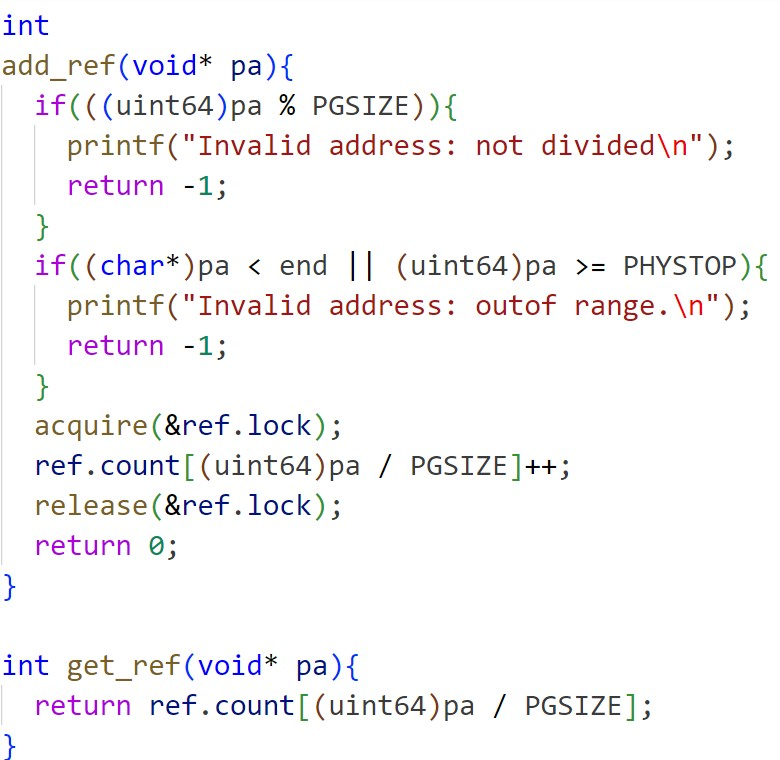
\includegraphics[height=8cm,width=7cm]{lab5-7.jpg}
\end{figure}\par

4.在trap.c中完善定义:主要分为修改usertrap,定义cow\_or\_not和定义cow\_lloc函数。\\
(1)修改usertrap,顺着上面的if(r\_scause==8)接着写一个else if,当r\_scause为12/13/15时,要进行COW的判断。
在下面新起的if语句中主要完成:对va判断是否超过PGSIZE;判断是不是COW页面,是会返回1;为这个进程分配页面,不返回0即可。否则就是异常情况(Tips-3),直接kill进程。
\begin{figure}[H]
    \centering
    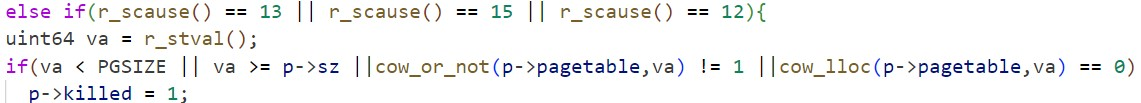
\includegraphics[height=2cm,width=13cm]{lab5-8.jpg}
\end{figure}

\noindent(2)完成对cow\_or\_not的定义。判断的依据就是PTE值,首先它应该和当前va映射的相同;并且要有PTE\_COW位。
\newpage
\begin{figure}[H]
    \centering
    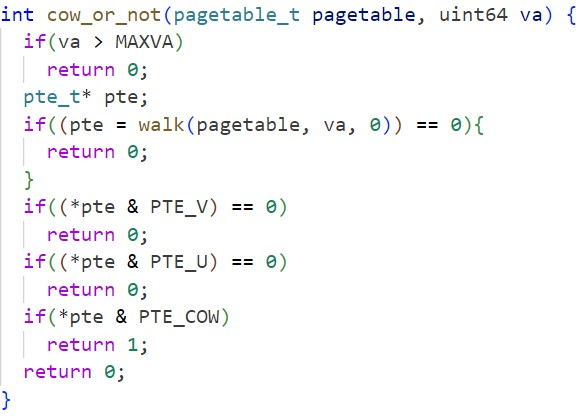
\includegraphics[height=6cm,width=7cm]{lab5-9.jpg}
\end{figure}
\noindent(3)完成cow\_lloc函数的定义。首先要得到物理地址pa和PTE,分别利用walkaddr函数和walk函数得到。接着我们对计数值进行判断;如果计数为1,皆大欢喜,直接开写权限,返回;如果不为1,就要分配一个新地址并且复制当前页面过去。
\begin{figure*}[!h]
    \centering
    \subfloat[get pa/PTE and ref == 1]{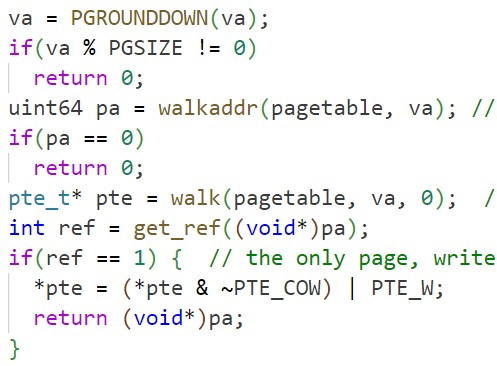
\includegraphics[width=7cm,height=5cm]{lab5-10.jpg} \label{X}}
    \hfill
    \subfloat[ref > 1]{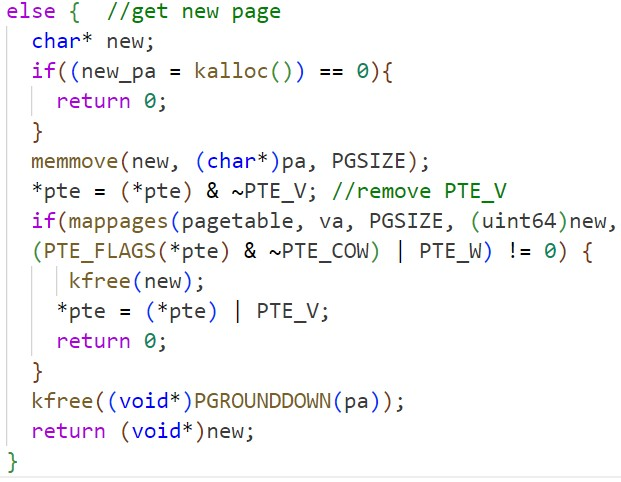
\includegraphics[width=7cm,height=7cm]{lab5-11.jpg} \label{Y}}
\end{figure*}


\begin{Large}
	\noindent 三、测试结果(make grade后得到的结果)
\end{Large}
\begin{figure}[H]
    \centering
    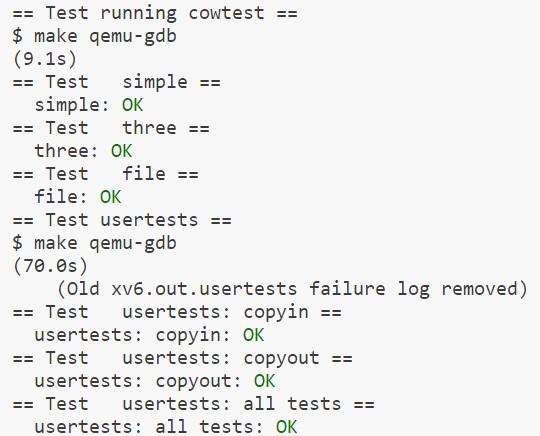
\includegraphics[height=5cm,width=6cm]{lab5-12.jpg}
\end{figure}
\end{document}